\documentclass{article}
\usepackage[utf8]{inputenc}
\usepackage{graphicx}
\usepackage{fancyhdr}
\usepackage{geometry}
\usepackage{amsmath}
\usepackage{amssymb}
\usepackage{algorithmicx}

\newcommand\tab[1][1cm]{\hspace*{#1}}
\geometry{left = 2.5cm, right=2.5cm, bottom=2.5cm, top=2.5cm}

\title{Ocuis - An Unnecessarily Convoluted Factorizor}
\author{Nick van der Merwe - s5151332 - nick.vandermerwe@griffithuni.edu.au}

\pagestyle{fancy}
\renewcommand{\headrulewidth}{1pt}
\fancyhf{}
\rhead{2803ICT - Assignment 2}
\chead{Griffith University}
\lhead{Nick van der Merwe - s5151332}
\rfoot{Page \thepage}

\begin{document}
    \maketitle

%==============================================================================

    \textit{Ocius - Latin. Swifter, more rapid}


    \section{Problem Statement}
    A server-client system is required where the server factorises 32 right
    rotated numbers and sends them to the client using shared memory.


    \section{User Requirements}
    From the user's perspective (the client) they should enter a number,
    then see the latest factor and the progress of each query.
    They should be able to enter a new query request at any time, except for
    when there are ten or more queries already running.
    In that case, a warning should pop up saying that it cannot take any input
    at the current moment.
    Additionally, once query finishes it announces that the query finished
    alongside how much time it took to do so.


    \section{Software Requirements}
    There should be two Cygwin compiled executables, server and client. Out
    of these the server should be launched first, and the user should launch
    the client and connect to the port.
    In terms of the requirements of the backend,
    \begin{enumerate}
        \item The client side should consist of either a single thread
        or multiple threads
        \item Unsigned 32-bit integers should be inputted - that is, the unsigned int
        type on a 64-bit machine
        \item The server will swap this into an unsigned long and open 32 threads
        for factorisation.
        Each one will be the original number rotated right - that is, if we insert 1
        its binary is ......001 and when its rotated it will be 100.....000 as
        it pushes it right and loops around to the start.
        In other words, the actual base-10 value will go 1 $\rightarrow 18*10^{18}$
        \item This will be factorised with the trial division method, and not the
        prime factors.
        It will return the actual factors and find them by finding the modulus
        less than the input of the input.
        \item The server should be able to run 10 queries at once (320 threads)
        \item The client reports responses instantly and when a query is complete
        the time will be reported
        \item Shared memory will be used between the server-client to manage the
        locks and conditionals.
        In the actual requirements, this is stated twice in two different ways.
        This solution uses a mix of both
        This handshake protocol will go into detail later
        \item The server is not allowed to use a buffer - it must be passed right away
        \item Originally the requirement is that the progress bar updates 500ms after
        an update from the server, but even with very large numbers this never occurs.
        Instead, the progress bar will update every 500ms.
        That should show both the requirement of measuring time and the progress bar,
        while being neat
    \end{enumerate}


    \section{Software design}
    This time we used C++, but only for classes and some STL.
    \subsection*{Diagram and overall algorithms}
    Earlier it was mentioned that the handshake protocol was replaced with a
    custom method.
    First, the original requirement is either redundant or contradicting -
    it was requested that integers are used to handle the read/write, then later
    down that mutexes and conditionals are used instead.  \\
    \tab
    This solution uses mutexes for the read/write, but integers as the conditionals.
    Due to the fact that conditionals are in fact built for buffered systems - or at
    least, every documentation example used a queue style structure - there
    is no wait on on the write side for when data is ready.
    Instead, a boolean is used to mark that the slot has been written into
    or read.
    \\ \tab Additionally, there is the tidbit of saying whether a slot is in use
    or not.
    For this, it was decided if a slot is holding 0, it means that it is not
    in use.
    While zero is a factor of zero, the trial division method would in fact crash if
    that input is given as the modulus operation would get called on a zero.
    So to notify the client that a socket is done, its set to zero.
    \\ \tab However, the client is single threaded and does not actually rely on this
    to find out that a slot is inactive.
    Every loop it searches over all the sockets for ones that are not zero and have
    their flags set that they need reading.
    \\ \tab The easiest way to communicate the overall algorithm is in a small diagram.
    \begin{figure}[ht!]
        \centering
        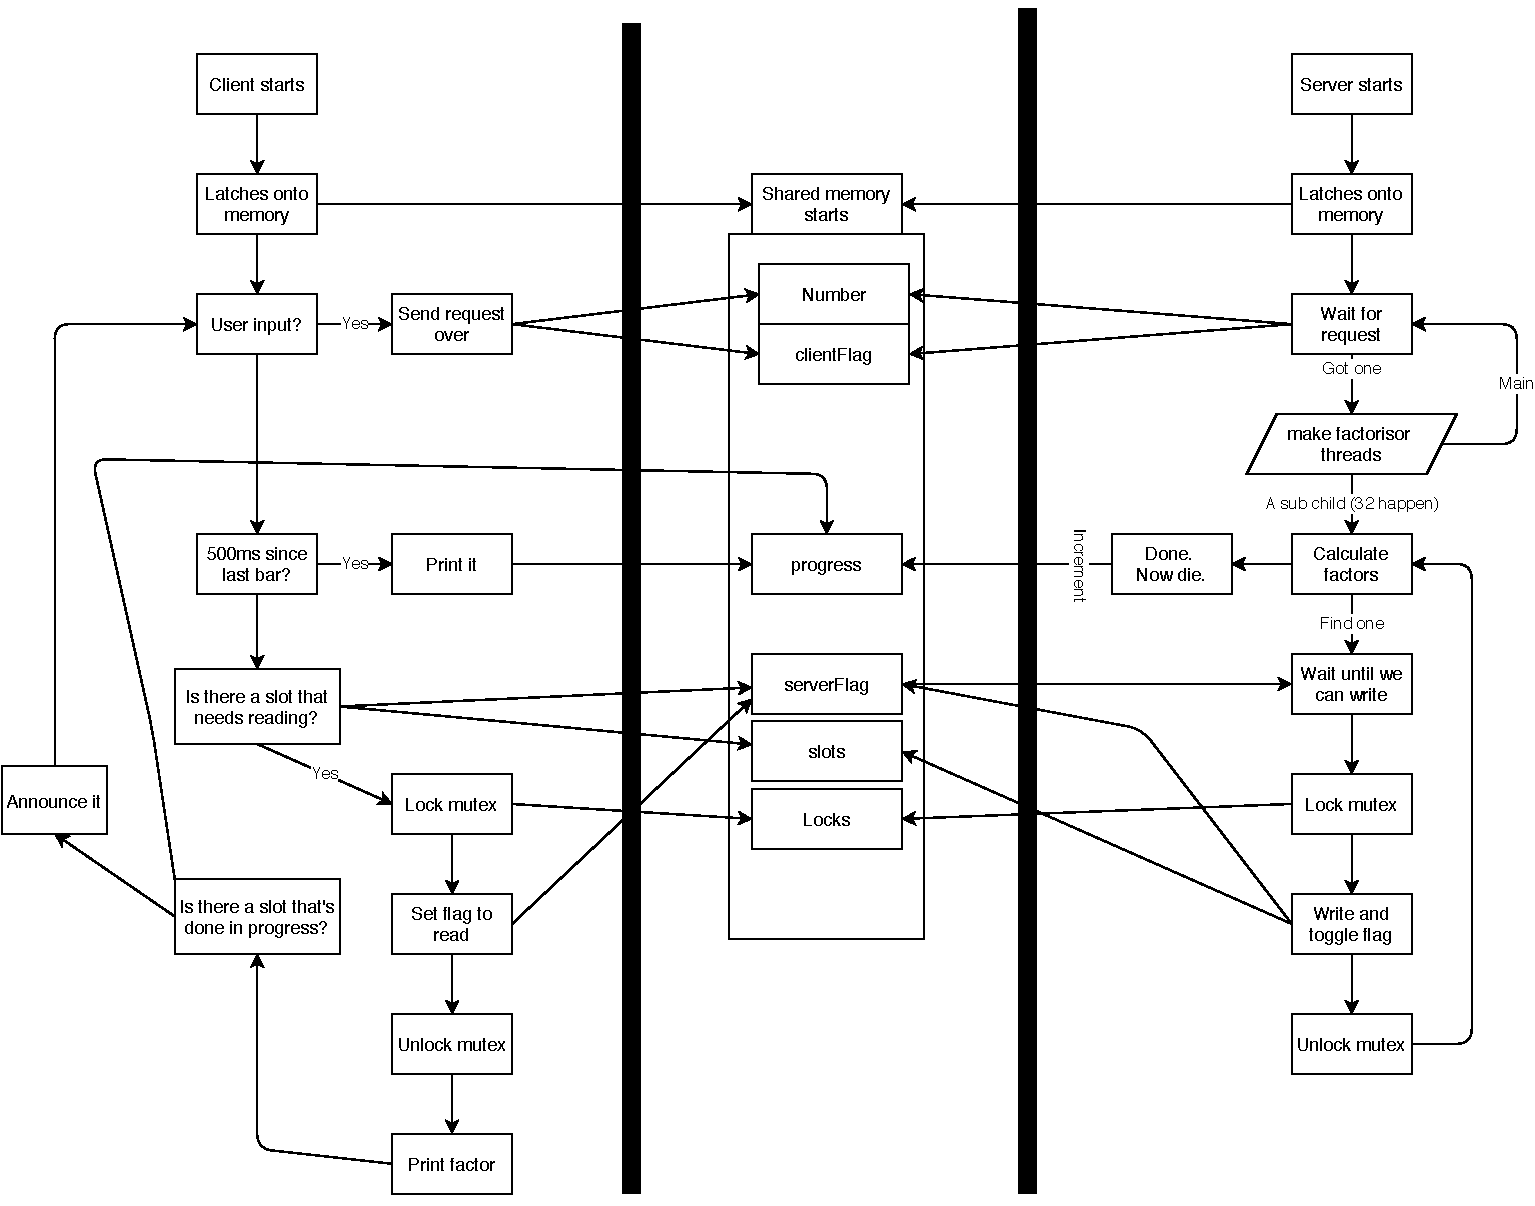
\includegraphics[scale=0.6]{figures/sharedMemoryModel.pdf}
        \caption{A small model of the program}
        \label{fig:sharedMemoryModel}
    \end{figure}
\newpage
    In terms of algorithms, there are no overly complicated ones. For clarification though,
    this is the method used for factorisation:
    \begin{figure}[ht!]
        \centering
        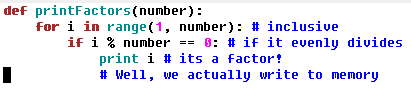
\includegraphics{figures/psuedoCode.png}
        \caption{Pseudo code for how factorisation is done}
        \label{fig:factorisation}
    \end{figure}

    \subsection*{Client}
    \subsubsection*{Clock class}
    This is basically just a custom clock class so that we can start a timer
    and finish it very cleanly from the outside perspective
    \begin{enumerate}
        \item void startTimer()
        \item bool isRunning() // returns a boolean for whether the clock
        was actually set
        \item double getSecondsAndDisable() // disables the boolean and calculates
        how many seconds passed since it was started
        \item private: timespecs and isCounting (whether its counting)
    \end{enumerate}
    %===========================================================================
    \subsubsection*{Shared memory class}
    This is so \textit{all} of the mutex operations, read and write function
    from the outside.
    Essentially, the idea is that you can just call readSlot() without doing
    any odd mutex operations from the outside perspective.
    On the client side here, it consists of:
    \begin{enumerate}
        \item SharedMemory() - the constructor.
        This latches on, or creates, the shared memory for us
        \item ~SharedMemory() - the destructor.
        Since this is the client side, we don't bother calling shmctl() or freeing
        our mutexes - that's the server's job when it shuts down.
        We just disconnect from the memory.
        \item requestReservation() - This handles finding a reservation for us,
        it waits until the clientFlag says we're allowed to write, then does so.
        \item grabReservationIndex() - Since the server can take a second
        to handle reservations, this is managed separately.
        It waits until the flag is set for reading, then grabs the reservation index.
        if it returned a value outside of [0, 9] then it tells the user that
        all the query slots are in use.
        \item readSlot() - This sets our lock, waits for the read flag to be set
        (however, it is only called when the read flag is set.
        This is a safety precaution)., reads the slot and sets the flag that it was set
        , then unlocks the mutex and returns the value it read.
        \item Subclass - shared data.
        This is the actual structure that exists in the shared memory. It
        contains everything we need - number, clientFlag, slots, progress,
        serverflag, and locks.
        \item Private things - key and shmid.
        These are to initialise the memory and its position
    \end{enumerate}

    \subsubsection*{Functions}
    \begin{enumerate}
        \item startingMessage() - This just prints the title screen and a number of newlines so
        that our escape character for moving up a line is functional
        \item readAnyNewFactors() - scans over the slots if anything can be read,
        and reads them. Reads one from every slot (if one is there)
        \item clearWaitForQuery() - Clears the warning message for waiting for a query
        \item sayQueryFinished() - Announces a query finished and how
        long it took to finish
        \item showProgressBar() - This manages printing the progress bar by
        checking the progress variable in the shared memory
        \item printWaitForQuery() - prints the warning message when a user
        attempts to type in a request for a query when 10 are already running
        \item handleAllPrints() - Runs through all the print functions for you.
        Requires a timer variable of the counts of all the timers for the sayQueryFinished()
        \item Main - Thanks to using select on our stdin to check for input, this
        got complicated.
        Essentially there's a select function which constantly checks if the user
        typed in any input, and then calls handleAllPrints() every loop to update
        all the information.
    \end{enumerate}
    \subsection*{Server side}
    \subsubsection*{SharedMemory}
    This is mostly the same as the client side of shared memory, however it has
    a few different functions:
    \begin{enumerate}
        \item SharedMemory() - the same as the client side, except we initialise
        the mutexes
        \item ~SharedMemory() - the same as the client side, except we free
        the mutexes and call shmctl() to delete it
        \item setToDefault() - Between runs it can occur that it just reuses
        the same shared memory as the previous client/server. This is a safety
        check that's enforced at the start of the program - it sets everything
        the default values again
        \item waitForReservation() - This waits until a flag is set by the client
        that a new query should start, and handles allocating it
        \item writeSlot() - This locks our mutex, waits for the write flag to get
        set, sets the write flag and writes the factor into the slot, and then locks
        the mutex again. We also have a 100 micro second pause here to slow down the program
        \item SharedData class - the same as the client
        \item Private variables are the same too
    \end{enumerate}
    \subsubsection*{Factorizor}
    This class handles all the threads and factorisation internally.
    Essentially we throw in a number and a memory index, then can go back to waiting
    for queries on the main thread.
    \begin{enumerate}
        \item Factorizer() ; ctor - This launches up 32 threads and
        specifically detaches them;
        that gives them permission to shut down on their own.
        We also have a sleep between each thread creation, because the data passed
        through $pthread\_t$ can have problems if it is too fast
        \item struct ThreadData() - This is the information each thread needs;
        which socket to write to and the number it needs to factorise
        \item static void * factoriseThread - This specifically needs
        to be a static function, without that inside of a class, pthread\_t has
        major problems.
        Those problems are also related to why the shared memory variables - flags
        specifically - were not just handled internally in the class.
    \end{enumerate}
    \subsubsection*{Functions}
    These are minimal compared to the client.
    \begin{enumerate}
        \item manageQuery() - takes in an index and launches up our factorizor
        \item startingMessage() - same as the client, except we
        don't have a number of newlines
        \item main() - We set our shared memory to default then wait for queries
        and call manageQuery() for each one
    \end{enumerate}

    \newpage
    \section{Detailed Software Testing}
    Everything works.
    \begin{figure}[ht!]
        \centering
        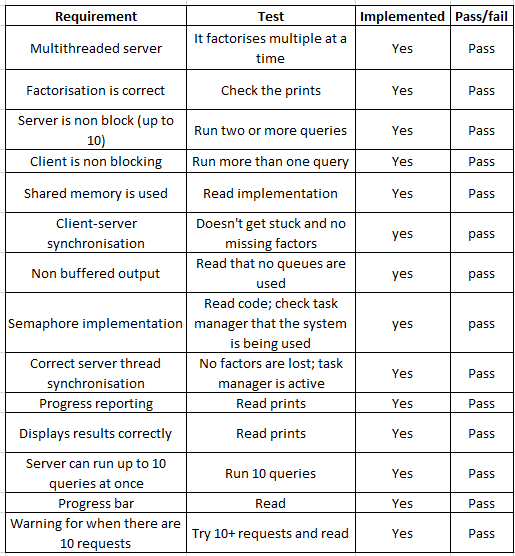
\includegraphics{figures/basicSoftwareTesting.png}
        \caption{Basic tests that it functions}
        \label{fig:basicTesting}
    \end{figure}

    \begin{figure}[ht!]
        \centering
        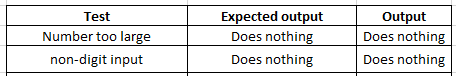
\includegraphics{figures/extensiveTests.png}
        \caption{Basic tests that it functions}
        \label{fig:extensiveTesting}
    \end{figure}


    \section{User Instructions}
    Compile with: \\
    \texttt{g++ server.cpp -o server -pthreads -O3} \\
    \texttt{g++ client.cpp -o client -pthreads -O3} \\
    and run \\
    \texttt{./server} \\
    \texttt{./client} \\
    Warning: Due to terminal differences and how specific some of the macros I use are,
    the output might not be as pretty for you as it is for me.
\end{document}
